\videotitle{Success Stories and Practical Recommendations}
%----------------------------------------------------------------------


\begin{frame}[c]{Large-scale Meta-Learning for HPO in Industry (Facebook)}

\begin{itemize}
    \item Facebook has an internal self-service machine learning (ML) system
    \myit{
    	\item Non-ML departments can integrate highly optimized ML models into their workflow
    	\item Hyperparameters of the ML models are optimized with Bayesian optimization
    }
\bigskip
\pause
    \item Training data for the models changes over time 
    \myit{
    	\item Hyperparameters are constantly re-optimized 
    	\item For efficiency: meta-learning Bayesian optimization, as described in \lit{\href{https://arxiv.org/abs/1802.02219}{Feurer et al. 2018}}
    }    
\medskip
    \begin{figure}
        \centering
        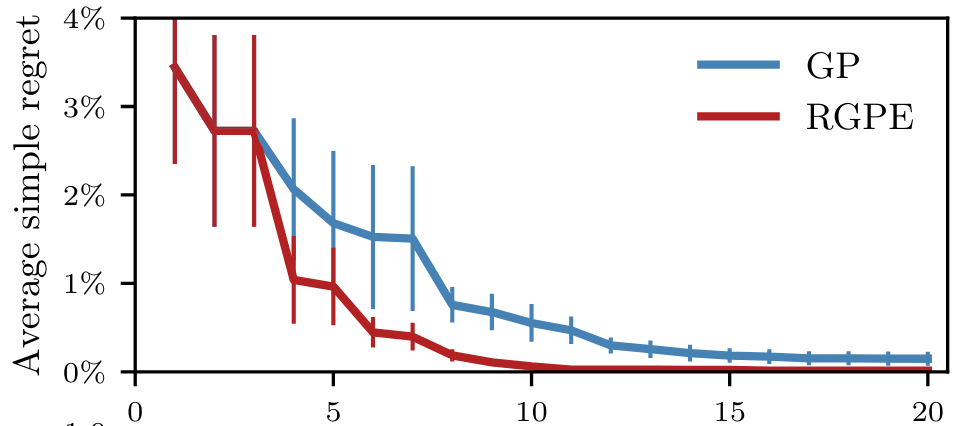
\includegraphics[width=0.5\textwidth]{../w07_hpo_speedup/images/success_stories/FB_RGPE.png}
        \caption{Bayesian optimization with meta-learning (RGPE) vs. vanilla Bayesian optimization (GP)}
    \end{figure}
\end{itemize}

\end{frame}

%-----------------------------------------------------------------------

\begin{frame}[c]{Auto-sklearn \litw{\href{https://papers.nips.cc/paper/5872-efficient-and-robust-automated-machine-learning}{Feurer et al, NIPS 2015}}}
Extension of Auto-WEKA with focus on speed improvements and robustness:
\begin{figure}
    \centering
    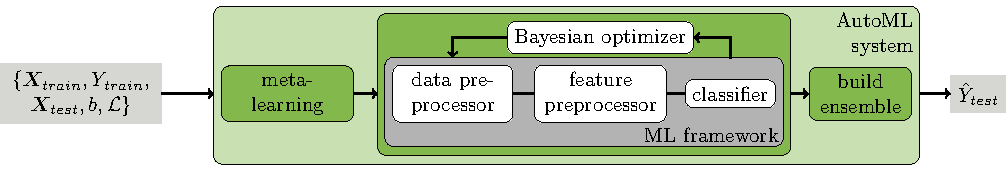
\includegraphics[width=0.9\textwidth]{images/success_stories/automlworkflow.pdf}
\end{figure}
\begin{itemize}
    \item Uses meta-learning to warmstart Bayesian optimization
\pause
    \item Won the 1st AutoML challenge
    \item Open source (BSD) and trivial to use 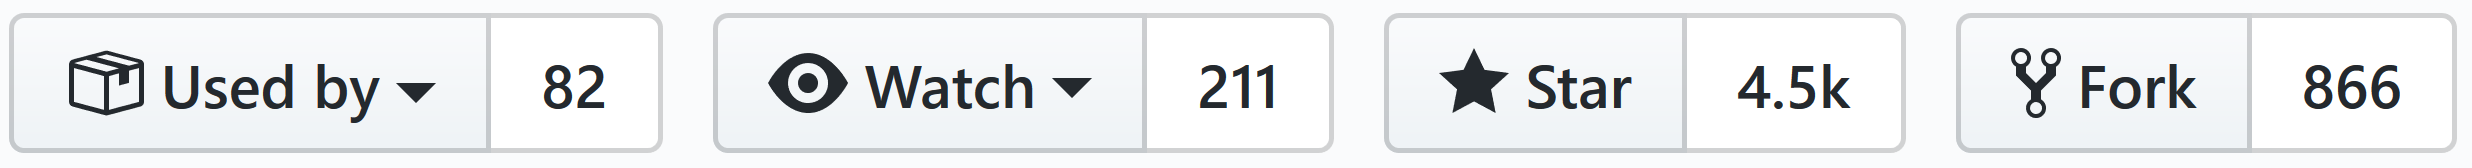
\includegraphics[width=0.5\textwidth]{images/success_stories/auto-sklearn-repo-stats.png}
\end{itemize}
\begin{figure}
    \centering
    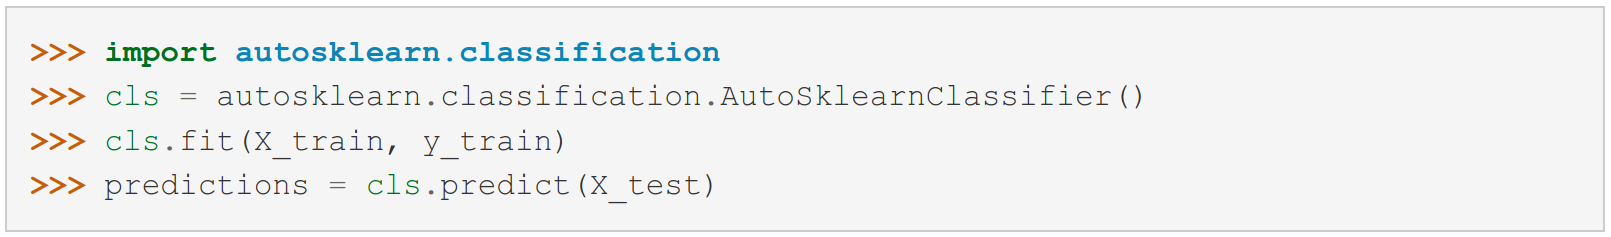
\includegraphics[width=0.85\textwidth]{images/success_stories/Auto-sklearn_01.png}
\end{figure}
\vspace*{-0.1cm}
Available at \url{https://automl.github.io/auto-sklearn}; frequently used in industry

\end{frame}

%-----------------------------------------------------------------------
\begin{frame}[c]{BOHB \litw{\href{http://proceedings.mlr.press/v80/falkner18a.html}{Falkner, Klein and Hutter, ICML 2018}}}

\myit{
	\item Robust and efficient 
	\item Only published in 2018, adopted by the community very quickly 
\begin{figure}
    \centering
    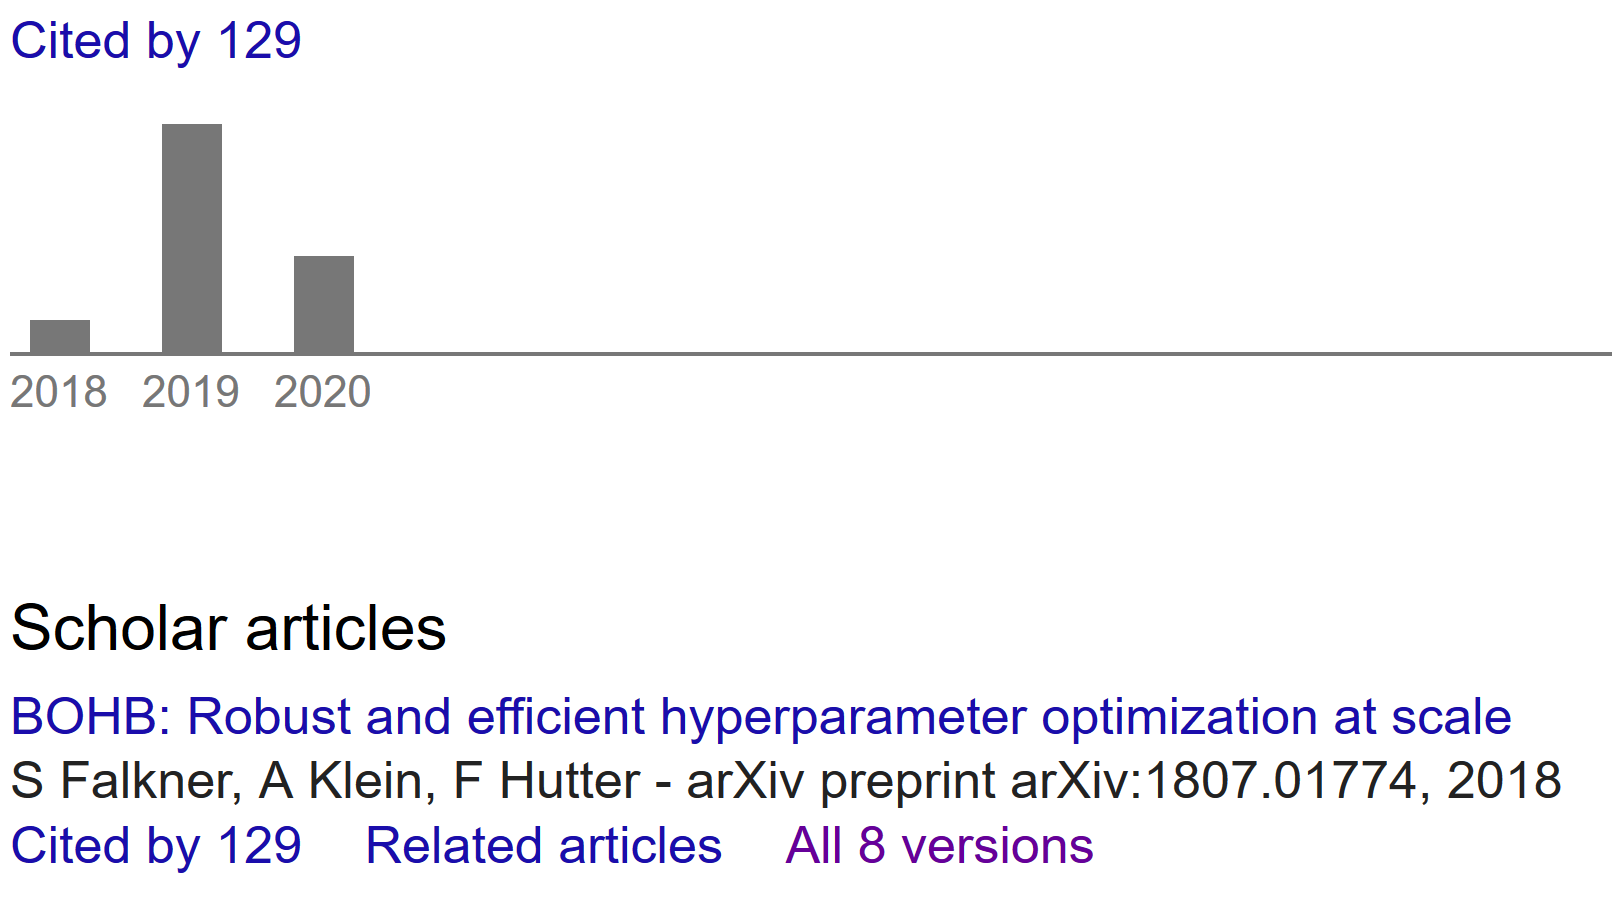
\includegraphics[height=4cm]{../w07_hpo_speedup/images/success_stories/BOHB-citations.png}
\end{figure}
\vspace*{0.4cm}
	\item Available at \url{https://github.com/automl/HpBandSter}
\begin{figure}
    
\includegraphics[height=0.6cm]{../w07_hpo_speedup/images/success_stories/BOHB-repo-stats.png}
\end{figure}
}

\end{frame}
%-----------------------------------------------------------------------

%-----------------------------------------------------------------------
\begin{frame}[c]{PoSH-Auto-sklearn \litw{\href{https://ml.informatik.uni-freiburg.de/papers/18-AUTOML-AutoChallenge.pdf}{Feurer et al. 2018}}}
Idea: integrate warmstarting and a BOHB-like approach for Auto-sklearn

\begin{figure}
    \centering
    \includegraphics[width=\textwidth]{images/success_stories/automl_bo_po_es.png}
\end{figure}
\pause

\begin{itemize}
    \item Uses task-independent meta-learning to warmstart Bayesian optimization
    \myit{
        \item Therefore, no need for (potentially unreliable) meta-features
    }
\pause
    \item Uses successive halving to quickly go through proposed configurations
    \myit{
        \item Therefore, scales better to larger datasets
    }
\pause
    \item Followed by BOHB-like approach (uses successive halving instead of Hyperband)
    \item Won the 2nd AutoML challenge
\end{itemize}

\end{frame}

%-----------------------------------------------------------------------
\begin{frame}[c]{Auto-sklearn 2.0}

\begin{columns}

\column{0.4\textwidth}
\vskip 35pt
Idea: automatically choose:
\begin{itemize}
    \item holdout or cross-validation
    \item optimization on the full budget or optimization with successive halving
\end{itemize}
using algorithm selection
\vskip 10pt
Yields huge improvements over Auto-sklearn 1.0.

\column{0.6\textwidth}
\begin{figure}
    \centering
    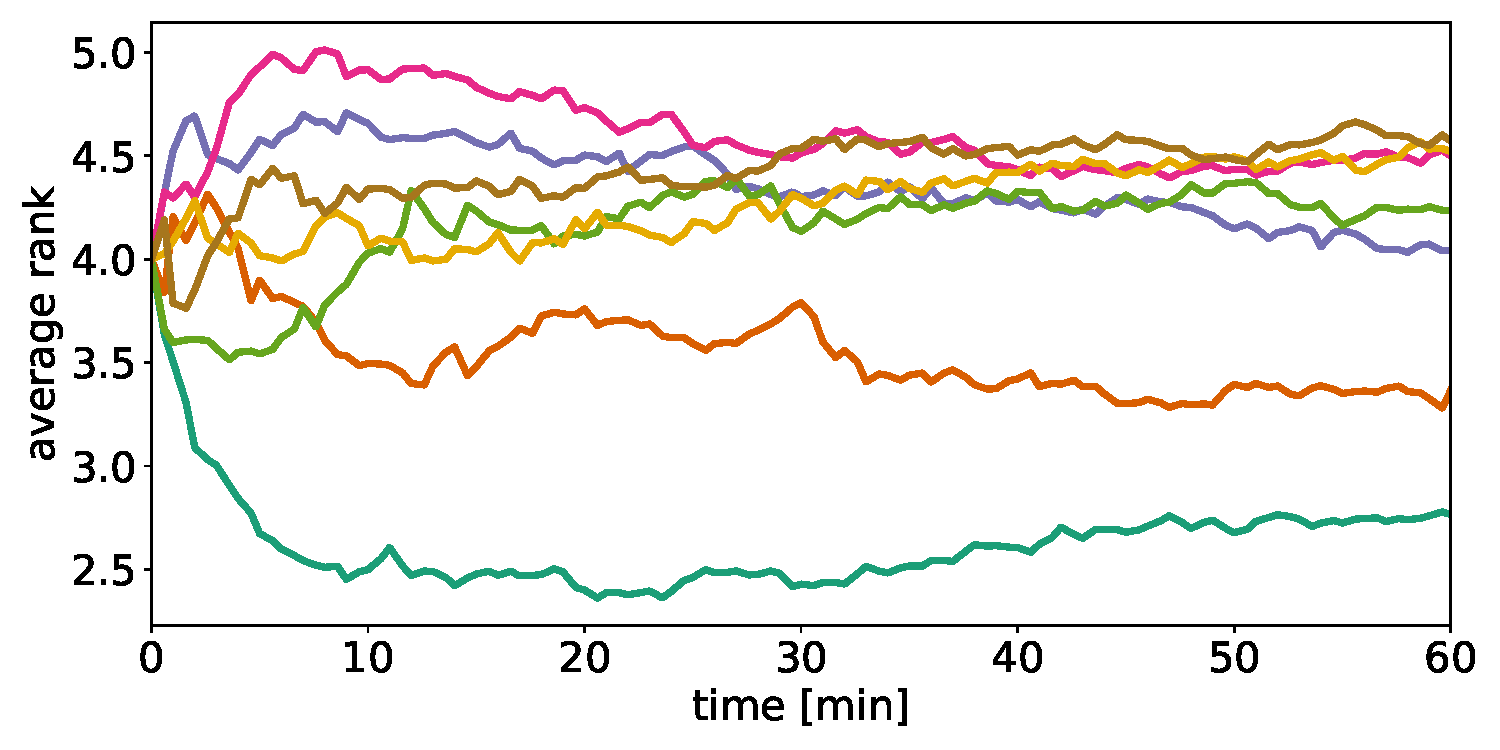
\includegraphics[width=\textwidth]{../w07_hpo_speedup/images/success_stories/RQ1_60MIN_ens_rank.pdf}
    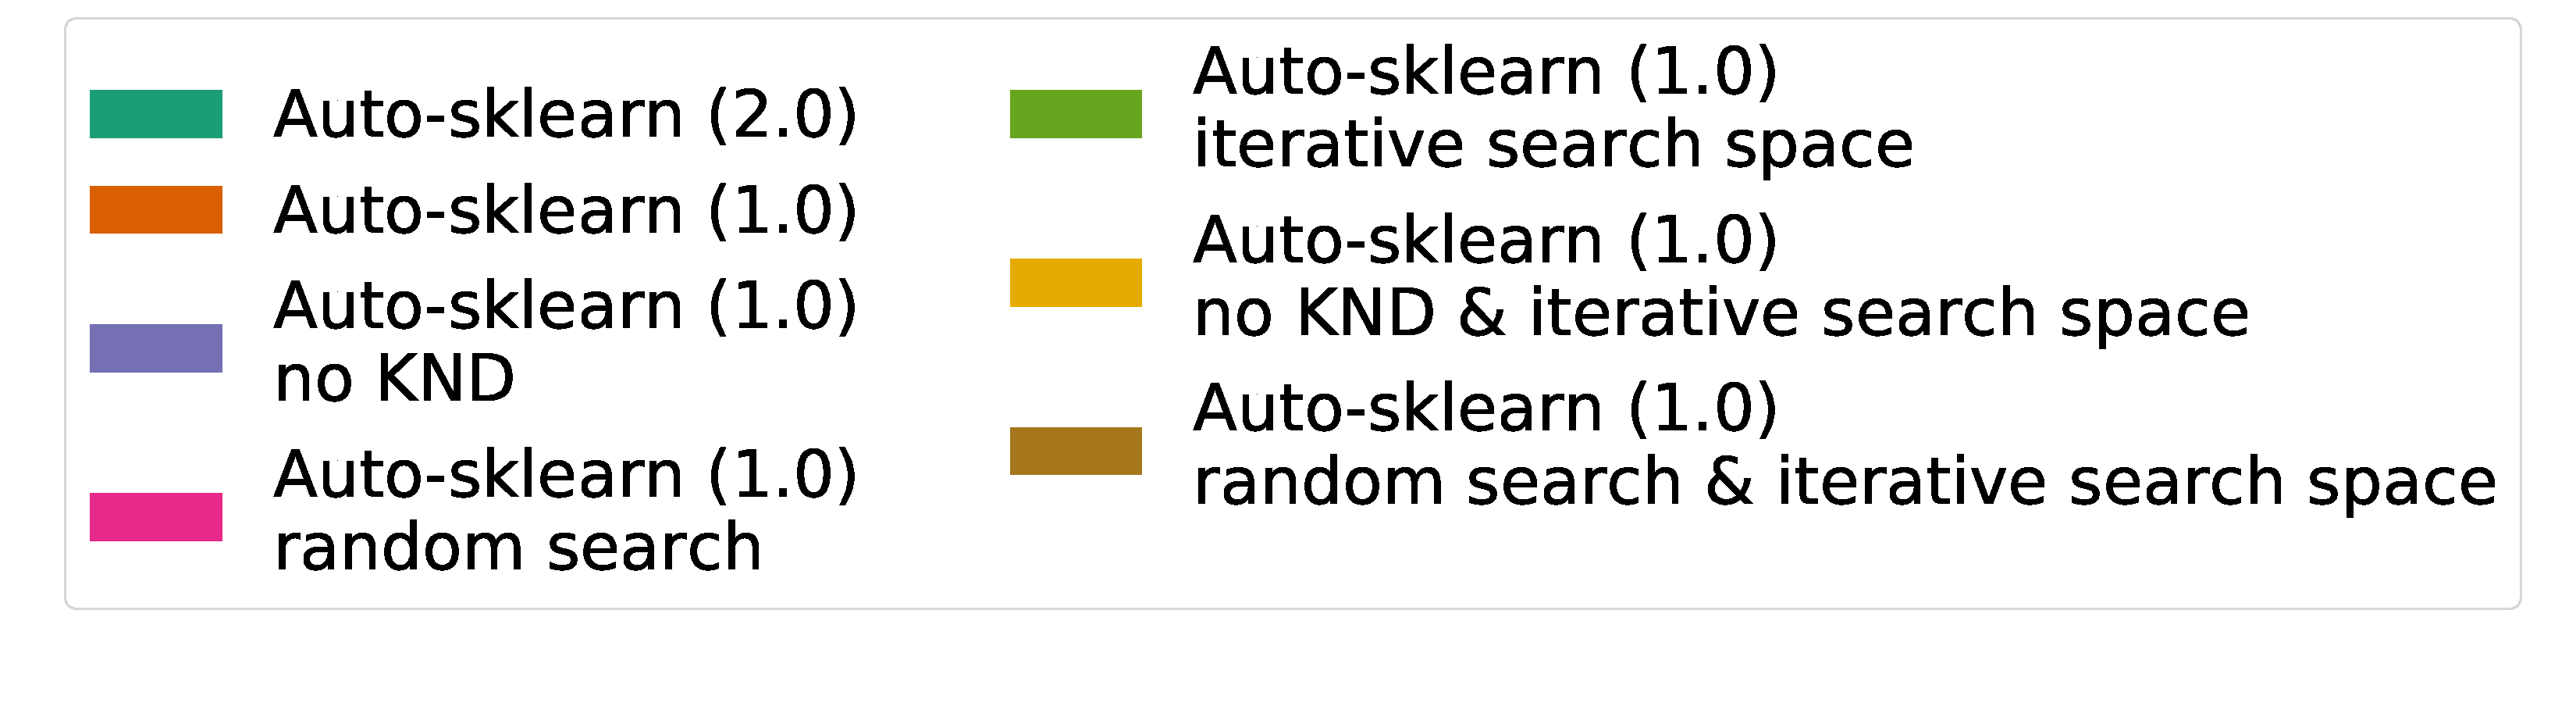
\includegraphics[width=\textwidth]{../w07_hpo_speedup/images/success_stories/RQ1_legend.pdf}
    \label{fig:my_label}
\end{figure}
\end{columns}

\end{frame}
%-----------------------------------------------------------------------

%-----------------------------------------------------------------------
\begin{frame}[c]{Practical Recommendations Which HPO Method to Use \litw{\href{https://link.springer.com/chapter/10.1007/978-3-030-05318-5_1}{Feurer \& Hutter, 2019}}}

\myit{
	\item If multiple fidelities available: BOHB \lit{\href{http://proceedings.mlr.press/v80/falkner18a.html}{Falkner, Klein and Hutter, ICML 2018}}
\bigskip
	\item Otherwise
	\myit{
		\item Low-dimensional continuous parameter space: 
		\myit{
			\item GP-based BO, e.g., Spearmint \lit{\href{https://papers.nips.cc/paper/4522-practical-bayesian-optimization-of-machine-learning-algorithms.pdf}{Snoek et al. 2012}}
		}
		\item High-dimensional discrete parameter space: 
		\myit{
			\item RF-based BO, e.g., SMAC \lit{\href{https://ml.informatik.uni-freiburg.de/papers/11-LION5-SMAC.pdf}{Hutter et al. 2011}}
		}
		\item Purely continuous, cheap function evaluations: 
		\myit{
			\item CMA-ES \lit{\href{https://arxiv.org/pdf/1604.00772.pdf}{Hansen et al., since 2001}};
%			\item Strong performance for HPO with large, parallel resources 
			evaluated for HPO by \lit{\href{https://arxiv.org/abs/1604.07269}{Loshchilov \& Hutter, ICLR WS 2016}}
		}
	}
}

\end{frame}
%-----------------------------------------------------------------------